\documentclass[titlepage,12pt,a4paper]{article}

\usepackage[left=2cm,top=3cm,right=2cm,bottom=3cm,bindingoffset=0.5cm]{geometry}
\usepackage{amsmath}
\usepackage{amssymb}
\usepackage{enumitem}
\usepackage{commath}
\usepackage{mathtools}
\usepackage{graphicx}
%\usepackage{csquotes}
%\usepackage{dirtytalk}
\usepackage{hyperref}
\usepackage{tabto}
\usepackage{gensymb}
\usepackage{graphicx}
\usepackage{listings}
\usepackage{sidecap}
\usepackage{wrapfig}
\usepackage{parskip}
\usepackage{units}

\usepackage{fancyhdr}
\usepackage{color}
\definecolor{dkgreen}{rgb}{0,0.6,0}
\definecolor{gray}{rgb}{0.5,0.5,0.5}
\definecolor{mauve}{rgb}{0.58,0,0.82}

\lstset{frame=tb,
  language=C++,
  aboveskip=3mm,
  belowskip=3mm,
  showstringspaces=false,
  columns=flexible,
  basicstyle={\small\ttfamily},
  numbers=left,
  numberstyle=\footnotesize,
  stepnumber=1,
  numbersep=5pt,
  keywordstyle=\color{blue},
  commentstyle=\color{dkgreen},
  stringstyle=\color{mauve},
  breaklines=true,
  breakatwhitespace=true,
  tabsize=3
}


\pagestyle{fancy}\lhead{A} \rhead{C}
\chead{{\large{\bf B}}}
\lfoot{}
\rfoot{\bf \thepage}
\cfoot{}

\setlength{\headheight}{15.2pt}
\pagestyle{fancy}
\fancyhf{}
\lhead{ \fancyplain{}{COMP3431: Robotic Software Architecture} }
\rfoot{ \fancyplain{}{\thepage} }


\begin{document}
\begin{titlepage}
    \begin{center}
        \vspace*{3cm}
        
        \Huge
        \textbf{COMP3431\\}
        \title{}
        \vspace{0.5cm}
        \Huge
        \textbf{Robotic Software Architecture}
        
        \vspace{0.54cm}
        
        \Large
        Assignment 2: Report
        
        \vspace{5cm}

	\large
	Nathan ADLER\\
	Aneita YANG\\

	\vfill
        
        \Large
        November 9, 2015
        
    \end{center}
\end{titlepage}

\pagebreak
\tableofcontents

\pagebreak
\section{Introduction}
In this assignment, both the hardware and software aspects of robotics are explored. The overall objective was to create a robot that could navigate autonomously in an outdoor environment, whilst avoiding any obstacles. An existing ground vehicle platform developed by student society CREATE UNSW was used as a base for testing.

To achieve the objective, the robot is equipped with a GPS and compass (using an Android phone with ROS). A laser scanner is also attached to the front of the robot, gathering information about the robot's immediate surroundings.

\subsection{Modules}

\subsubsection{Hardware}

The Unmanned Ground Vehicle (UGV) was developed to serve as an autonomous platform for the research and testing of robotic systems. It measures \unit[1]{m} long, and weighs approximately \unit[50]{kg}. The robot was constructed using parts from an electric wheelchair and a custom-design welded steel chassis. The following hardware is contained on board:
\begin{itemize}
	\item Dell Latitude E6400 notebook
	\item SICK TiM551 2D laser scanner
	\item DLink DSL 2750B N300 Modem Router
	\item Sony Xperia Z3 compact
	\item Arduino Mega 2560 R3
	\item Sabertooth 2X25 regenerative motor driver
	\item 2 x 12V lead acid battery
	\item 2 x electric wheelchair motor
\end{itemize}

The Dell notebook was installed with Ubuntu 14.04 (a.k.a. "Trusty Tahr") and ROS Indigo. Sensors from the phone and laser scanner were integrated in a Local Area Network through a combination of ethernet and wireless connections. A SSH tunnelling engine was installed to allow for remote communication over the internet between enabled devices, including a precise positioning GPS device developed for an undergraduate thesis. 

\begin{figure}[h!]
	\centering
	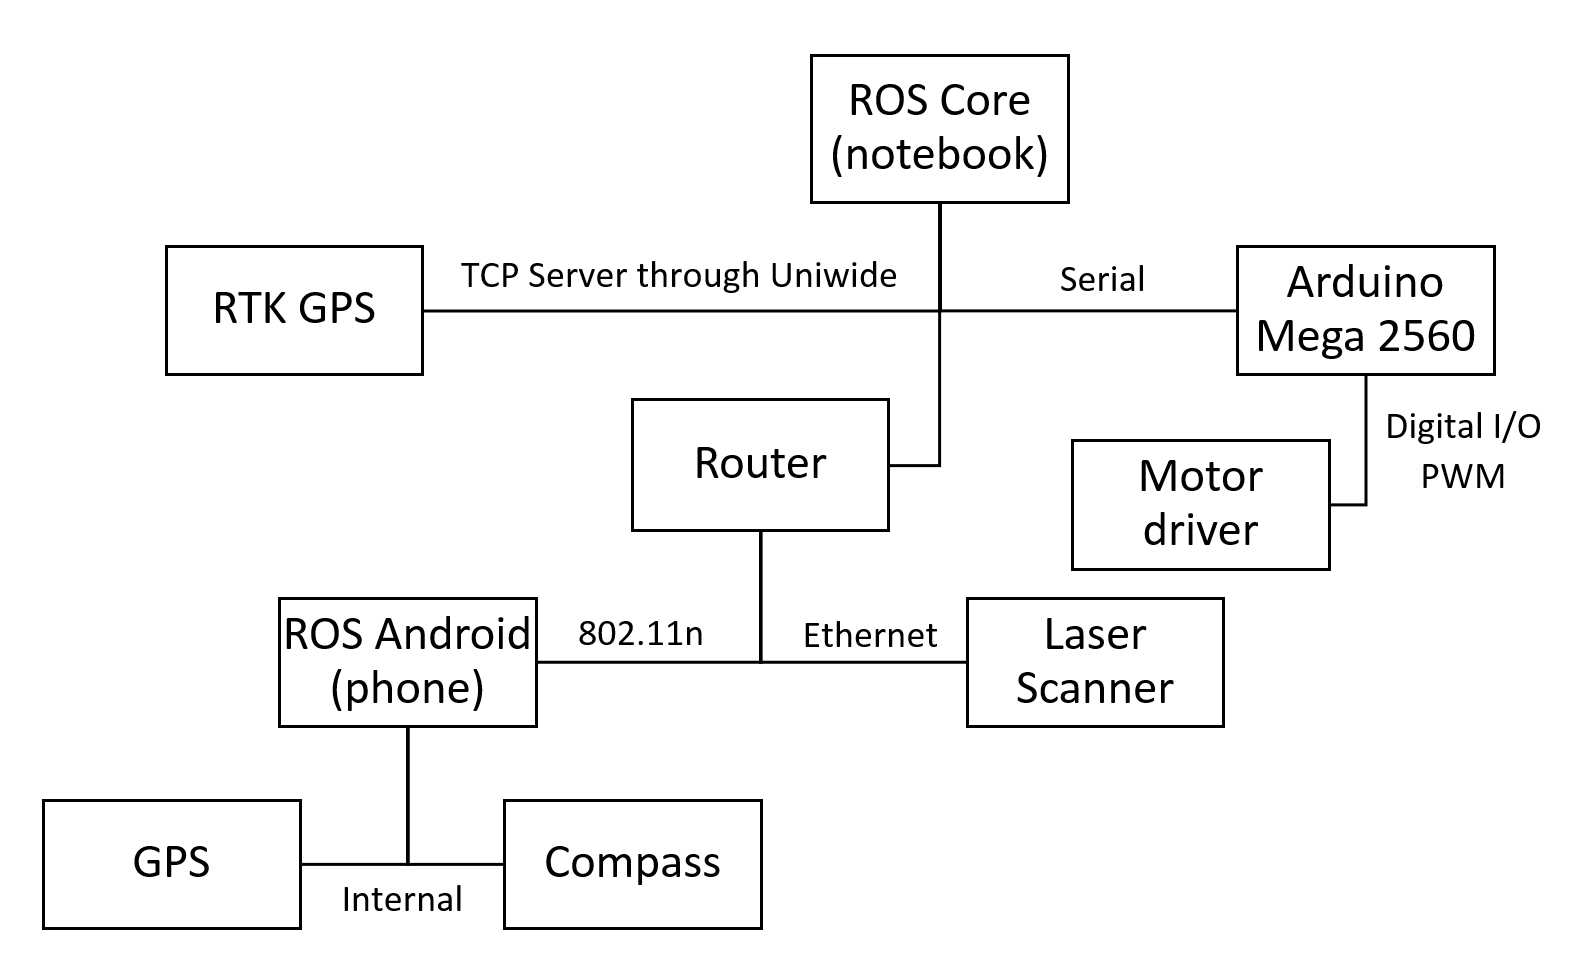
\includegraphics[scale=0.6]{figures/hardware_chart.png}
	\caption{Hardware map of UGV}
	\label{figure:hardware_chart}
\end{figure}
\pagebreak

\subsubsection{Software}

On the software side, five/six(?????) nodes run in conjunction to operate the robot:

\verb|dest_sender| keeps track of the robot's remaining waypoints.

\verb|gps_drive| calculates and publishes the direction in which the robot needs to travel to reach its destination.

\verb|rtk_gps_pub| publishes the an optional precise position based on real time kinematic GPS solutions with centimetre-level accuracy.

\verb|laser_safe| publishes movement messages, either directly to the bot's destination, or to avoid an obstacle.

\verb|motordata_arduino_send| converts movement messages into serial messages to send to the Arduino that controls the motord driver and drives the robot.

\verb|sick_tim| reads data from the SICK TiM551 2D laser scanner and publishes the data as a \verb|laser_scan| ROS message.

\pagebreak

\subsection{Planner}
The planner module is responsible for keeping track of the robot's waypoints and informs the robot of its next destination. 

The \verb|dest_sender| node parses a file containing the GPS coordinates of waypoints and turns each latitude-longitude pair into a NavSatFix message. Each waypoint is stored in a list (as a NavSatFix message), with the head of the list being the robot's next destination. \verb|dest_sender| publishes this message to the \verb|/ugv_nav/waypoints| topic for other modules to subscribe to.

\verb|dest_sender| subscribes to the \verb|/ugv_nav/arrived| topic, which signals when the robot has reached its destination. Messages which are published to the \verb|/ugv_nav/arrived| topic trigger a callback which removes the current waypoint from the list (i.e. the head of the list). If the robot has not reached its final destination and the list is not empty, the robot's next destination is published.

\subsection{Localisation}
The localisation module is responsible for calculating the heading from the robot's current position to its destination and determines a direction in which the robot should travel to reach its goal.

To assist with the autonomous driving, the robot is equipped with an Android phone running the \verb|android_sensors_driver| app which publishes:

\begin{itemize}
	\item Camera images: \verb|sensor_msgs/CompressedImage| and \verb|sensor_msgs/Image|
	\item Fluid pressure data: \verb|sensor_msgs/FluidPressure|
	\item Illuminance data: \verb|sensor_msgs/Illuminance|
	\item Accelerometer: \verb|sensor_msgs/Imu|
	\item Magnetic field: \verb|sensor_msgs/MagneticField|
	\item GPS fixes: \verb|sensor_msgs/NavSatFix|
	\item Temperature data: \verb|sensor_msgs/Temperature| \\
\end{itemize}

For the purposes of this assignment, data gathered from the phone's GPS fixes and magnetic fields are used to calculate the bearing of the destination from the robot. The \verb|gps_drive| node performs these calculations - the Android device publishes the GPS coordinates of the robot to the \verb|/phone1/android/fix| topic and the GPS coordinates of the destination are published to the \verb|/ugv_nav/waypoints| topic by the \verb|dest_sender| node. The Android device also publishes information about the robot's bearings to \verb|/phone1/android/magnetic_field|.

\begin{align*}
	\text{difference\_lat}   	&= 	\text{destination\_latitude} - \text{source\_latitude} \\
	\text{difference\_long}	&= 	\text{destination\_longitude} - \text{source\_longitude} \\
\end{align*}

Supposing the robot is facing true north, then:
\begin{align*}
	\theta	&=	\tan^{-1}({\frac{\text{difference\_long}}{\text{difference\_lat}}}),\\
\end{align*}
where $\theta$ is the angle the robot must turn to reach its destination.

\begin{figure}[h]
	\centering
	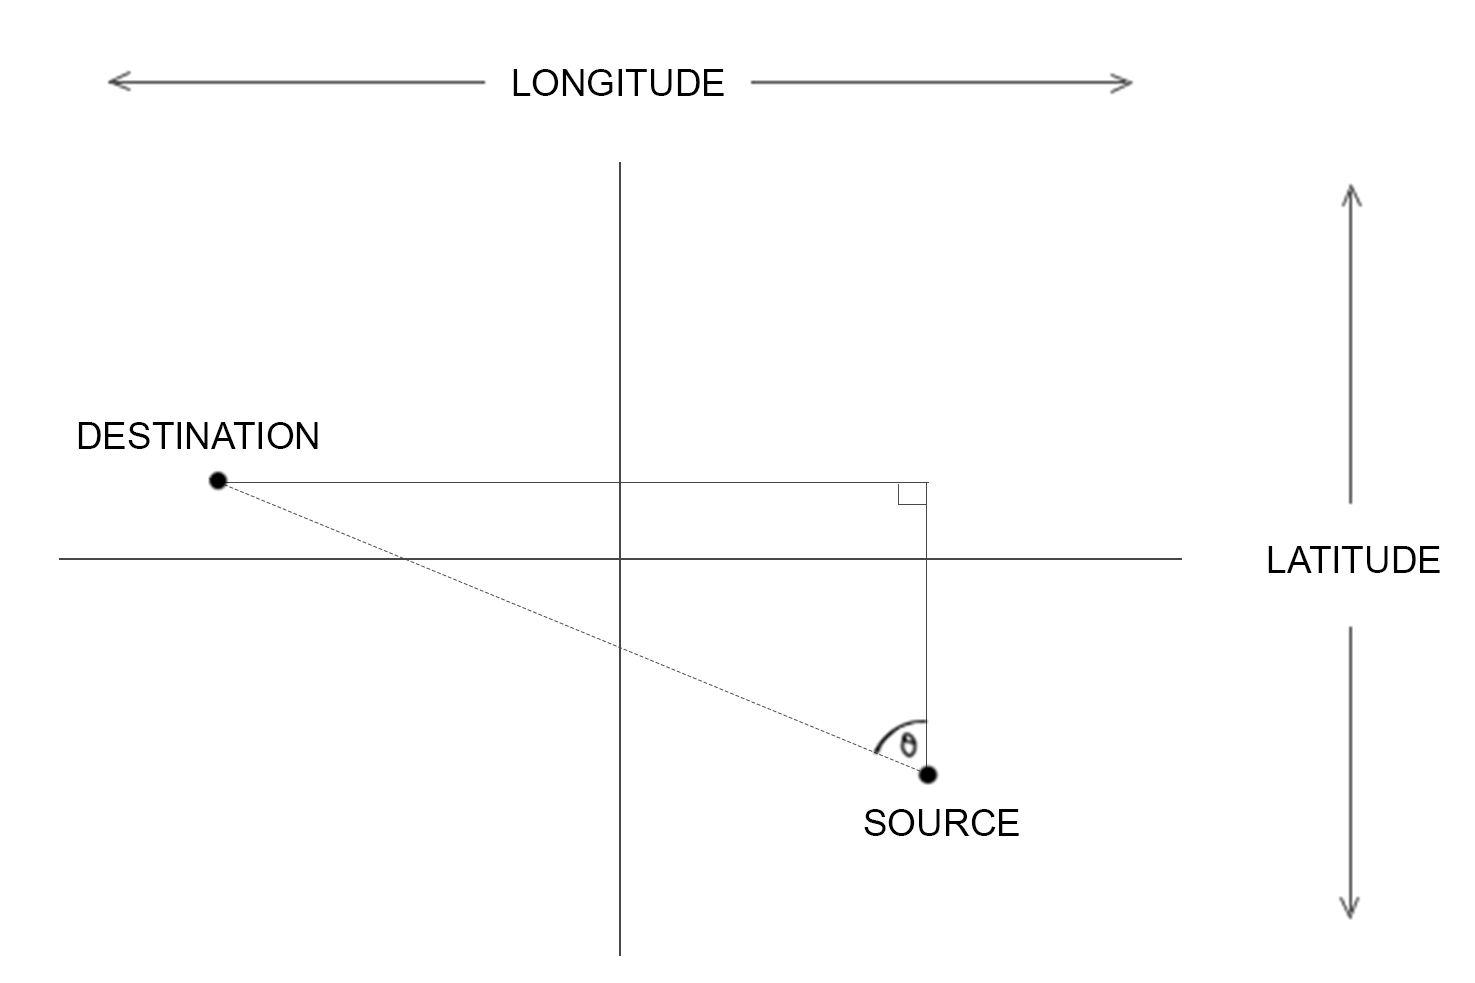
\includegraphics[scale=1]{bearings.png}
	\caption{Calculation of the bearing of the destination from the robot, if the robot is facing true north.}
\end{figure}

\text{As the ???th decimal place provides up to ??? precision:}

\begin{align*}
	\text{distance\_to\_destination}	&= 	111,000 * \sqrt{(\text{difference\_lat})^2 + (\text{difference\_long})^2}
\end{align*}

If the distance to the destination is less than 5 (i.e. the robot is within 5 metres of its destination), it is considered to have arrived at its destination. At this stage, the \verb|gps_drive| node will publish a message to the \verb|/ugv_nav/arrived| topic, signalling to the \verb|dest_sender| that the robot has reached its destination and that a new destination is required.

As the robot obtains GPS fixes frequently, it is sensitive to small changes to its position. The frequent updating of the robot's position results in abrupt movement changes as the robot attempts to face the bearing to its destination. In order to reduce the amount of sudden directional changes, rather than continually looking for a straight, direct path to its goal, the direction the robot decides to travel is biased towards a `smooth path'.

TODO: Explain straight line bias calculations 

\subsection{Waypoint Traversal}
lasersafe, motordata

\subsection{Open Source SICK TiM Driver}

\pagebreak
\section{Results}

\pagebreak
\section{Future Work and Improvements}

\pagebreak
\section{Appendix}


\subsection{sensor\_msgs/NavSatFix.msg}
\begin{lstlisting}[language=C++]
Header header

/* Satellite fix status information */
NavSatStatus status

/* Latitude [degrees]. Positive is north of equator; negative is south. */
float64 latitude

/* Longitude [degrees]. Positive is east of prime meridian; negative is west. */
float64 longitude

/*
Altitude [m]. Positive is above the WGS 84 ellipsoid
(quiet NaN if no altitude is available).
*/
float64 altitude

/*
Position covariance [m^2] defined relative to a tangential plane
through the reported position. The components are East, North, and
Up (ENU), in row-major order.
Beware: this coordinate system exhibits singularities at the poles.
*/
float64[9] position_covariance

/*
If the covariance of the fix is known, fill it in completely. If the
GPS receiver provides the variance of each measurement, put them
along the diagonal. If only Dilution of Precision is available,
estimate an approximate covariance from that.
*/
uint8 COVARIANCE_TYPE_UNKNOWN = 0
uint8 COVARIANCE_TYPE_APPROXIMATED = 1
uint8 COVARIANCE_TYPE_DIAGONAL_KNOWN = 2
uint8 COVARIANCE_TYPE_KNOWN = 3

uint8 position_covariance_type
\end{lstlisting}


\end{document}
